\chapter{Control as Inference}
In this chapter, we will talk about how we derive optimal control, reinforcement learning, and planning as
probabilistic inference. In a lot of scenarios that, say, involve biological behaviors, the data is not optimal. The behavior of the agent might be stochastic, but good behaviors are still more likely. 

\section{Probabilistic Graphical Model of Decision Making}
When we do not make any assumption of optimal behavior, we cannot ensure that the actions are chosen optimally. In other words, we cannot assume the following relation:
\[
a_1,\dots,a_T = \argmaxA_{a_1,\dots,a_T}\sum_{t=1}^Tr(s_t,a_t)
\]
Instead, we should model the probability distribution of seeing a trajectory $p(\tau) = p(s_{1:T},a_{1:T})$. We also introduce a binary optimality variable $\mathcal{O}_t$, which represents if the agent if behaving optimally at time step $t$. Then we are interested in $p(\tau|\mathcal{O}_{1:T})$, where we infer the probability of the given trajectory given the agent is optimal at every time step.
\begin{figure}
    \centering
    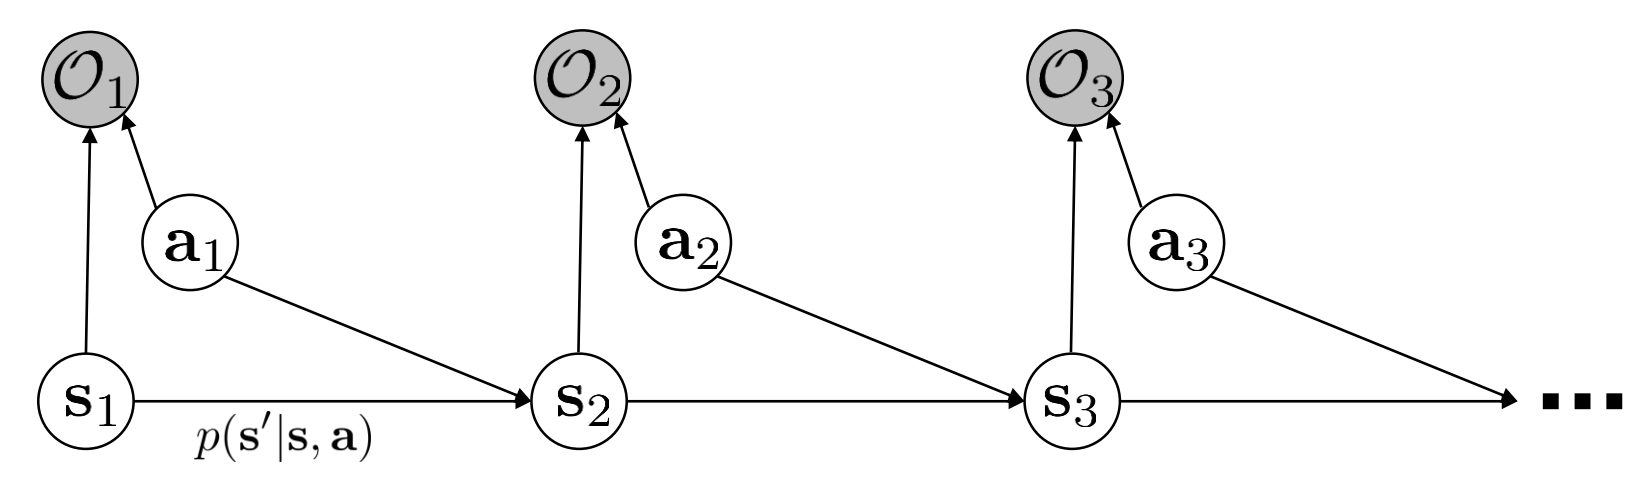
\includegraphics[scale=0.4]{figures/opt.png}
    \caption{Optimalility in stochastic behaviors}
    \label{fig:opt}
\end{figure}
Now we will model the optimality variable as follows: we model that the probability that variable is true given state and action is an exponential of the reward:
\[
p(\mathcal{O}_t|s_t,a_t) = \exp{r(s_t,a_t)}
\]
this might seem an arbitrary choice at the first sight, but we shall see later that this gives us an elegant mathematical expression in our derivation. We also assume for now that the reward function is always negative, but we can always take any reward function and normalize it by subtracting the max reward. Then by Bayes' Rule, we have:
\begin{align*}
    p(\tau|\mathcal{O}_{1:T}) &= \frac{p(\tau,\mathcal{O}_{1:T})}{p(\mathcal{O}_{1:T})}\\
    &\propto p(\tau)\prod_t \exp{r(s_t,a_t)}\\
    &= p(\tau)\exp{\sum_t r(s_t,a_t)}
\end{align*}
What does the above expression imply? Well, let us pretend that the dynamics are deterministic, then the first term $p(\tau)$ just means if this trajectory is possible. If not, then the probability is 0. If the trajectory is indeed possible, since we are multiplying by the exponent of the sum of rewards, then the probability of a trajectory given the agent is acting optimally is big with high rewards, but small with low rewards.

Let us take a look at the optimality model in Fig. \ref{fig:opt}. Why is this model important? Because the model is able to model suboptimal behavior, which is important for inverse RL that will be covered later. We then can apply inference algorithms to solve control and planning problems. It also provides an explanation for why stochastic behavior might be preferred, which is useful for exploration and transfer learning.

\subsection{Inference in the Optimality Model}
The first inference we will do is to compute the backward message $\beta_t(s_t,a_t) = p(\mathcal{O}_{t:T}|s_t,a_t)$, which means the probability of the agent being optimal from the current time step to the end given state and action. Another inference we will do is the policy $p(a_t|s_t,\mathcal{O}_{1:T})$. Note that we are inferring the possible actions taken given optimality. The last inference we do is the forward message $\alpha_t(s_t) = p(s_t|\mathcal{O}_{1:t-1})$, which is the probability of landing in a particular state given that the agent is acting optimally up to the current time step. 

\subsection{Inferring the Backward Messages}
The backward messages we are inferring is $\beta_t(s_t,a_t) = p(\mathcal{O}_{t:T}|s_t,a_t)$, which we will try to express in terms of transition probability $p(s_{t+1}|s_t,a_t)$ and optimality probability $p(\mathcal{O}_t|s_t,a_t)$. Mathematically, we can calculate $\beta_t(s_t,a_t)$ as:
\begin{align*}
    \beta_t(s_t,a_t)&=p(\mathcal{O}_{t:T}|s_t,a_t)\\
    &= \int p(\mathcal{O}_{t:T},s_{t+1}|s_t,a_t)ds_{t+1}\\
    &= \int p(\mathcal{O}_{t+1:T}|s_{t+1})p(s_{t+1}|s_t,a_t)p(\mathcal{O}_{t}|s_t,a_t)ds_{t+1}
\end{align*}
The second and the third terms in the product are known, so let us now focus on the first term:
\begin{align*}
p(\mathcal{O}_{t+1:T}|s_{t+1}) &= \int p(\mathcal{O}_{t+1:T}|s_{t+1},a_{t+1})p(a_{t+1}|s_{t+1})da_{t+1}\\
&=\int \beta(s_{t+1},a_{t+1})da_{t+1}
\end{align*}
we ignored $p(a_{t+1}|s_{t+1})$ it means which actions are likely a priori, and we assume it is uniform (constant) for now.

Therefore, to calculate the backward message, we have a recursive relation. For $t= T-1\;\text{to}\;1$:
\begin{align*}
    \beta_t(s_t,a_t) &= p(\mathcal{O}_{t}|s_t,a_t)\mathbb{E}_{s_{t+1}\sim p(s_{t+1}|s_t,a_t)}[\beta_{t+1}(s_{t+1})]\\
     \beta_t(s_t) &= \mathbb{E}_{a_{t}\sim p(a_t|s_t)}[\beta_t(s_t,a_t)]
\end{align*}

\subsection{A Closer Look}
Let us take a closer look at the backward pass. Let $V_t(s_t) = \log \beta_t(s_t)$, and let $Q_t(s_t,a_t) = \log \beta_t(s_t,a_t)$. Then 
$$V_t(s_t) = \log \int \exp (Q_t(s_t,a_t))da_t$$
As $Q_t(s_t,a_t)$ gets bigger $V_t(s_t)\rightarrow \max_{a_t}Q_t(s_t,a_t)$. Using the expression of $\beta_t(s_t,a_t)$, we will have
\[
Q_t(s_t,a_t) = r(s_t,a_t) + \log \mathbb{E}[\exp (V_{t+1}(s_{t+1}))]
\]

Recall in value iteration, we set $Q(s,a) \leftarrow r(s,a) + \gamma \mathbb{E}[V(s')]$. When the transition is deterministic, we have $Q_t(s_t,a_t) = r(s_t,a_t)+V_{t+1}(s_{t+1})$, which is similar to value iteration. However, when the transition is stochastic, then the $\log \exp$ term is like a maximum operation, so we have a biased optimistic estimation of the Q-function.

\subsection{Aside: The Action Prior}
Recall that we assumed $p(a_t|s_t)$ to be uniform, so it became constant in our integral. However, we shall see that it does not change much if the action prior is not uniform. Our V function now becomes $V_t(s_t) = \log \int \exp (Q_t(s_t,a_t)+\log p(a_t|s_t))da_t$, and our Q-function becomes $Q(s_t,a_t) = r(s_t,a_t) + \log p(a_t|s_t) + \log \mathbb{E}[\exp (V_{t+1}(s_{t+1}))]$
We can put the extra $p(a_t|s_t)$ into the reward term, then we will have the same expression of the Q-funtion, thus the V function. Therefore, uniform action prior can be assumed without loss of generality because it can always be folded into the reward.

\subsection{Inferring the Policy}
Now with backward messages available to us, we can then proceed to infer the policy $p(a_t|s_t,\mathcal{O}_{1:T})$. We derive the policy as follows:
\begin{align*}
    p(a_t|s_t,\mathcal{O}_{1:T}) &= \pi(a_t|s_t)\\
    &= p(a_t|s_t,\mathcal{O}_{t:T})\\
    &= \frac{p(a_t,s_t|\mathcal{O}_{t:T})}{p(s_t|\mathcal{O}_{t:T})}\\
    &= \frac{p(\mathcal{O}_{t:T}|a_t,s_t)p(a_t,s_t)/p(\mathcal{O}_{t:T})}{p(\mathcal{O}_{t:T}|s_t)p(s_t)/p(\mathcal{O}_{t:T})}\\
    &= \frac{p(\mathcal{O}_{t:T}|a_t,s_t)}{p(\mathcal{O}_{t:T}|s_t)}\frac{p(a_t,s_t)}{p(s_t)}\\
    &= \frac{\beta_t(s_t,a_t)}{\beta_t(s_t)}p(a_t|s_t)
\end{align*}
we discard the optimality variables $1,\dots t-1$ because then are conditionally independent of $s_t$. We also discard $p(a_t|s_t)$ since we can assume it as uniform. Using the definition of $V,Q$, we have
\begin{align*}
    \pi(a_t|s_t)&= \frac{\beta_t(s_t,a_t)}{\beta_t(s_t)}\\
    &= \exp(Q_t(s_t,a_t) - V_t(s_t))\\
    &= \exp(A_t(s_t,a_t))
\end{align*}
This result makes sense, because when we have large advantage function values, the action is more likely to be taken.

\subsection{Inferring the Forward Messages}
We now can infer our third task, the forward message $\alpha_t(s_t) = p(s_t|\mathcal{O}_{1:t-1})$. The derivation is as follows:
\begin{align*}
    \alpha_t(s_t) &= p(s_t|\mathcal{O}_{1:t-1})\\
    &= \int p(s_t,s_{t-1},a_{t-1}|\mathcal{O}_{1:t-1})ds_{t-1}da_{t-1}\\
    &= \int p(s_t|s_{t-1},a_{t-1},\mathcal{O}_{1:t-1})p(a_{t-1}|s_{t-1},\mathcal{O}_{1:t-1})p(s_{t-1}|\mathcal{O}_{1:t-1})ds_{t-1}da_{t-1}\\
    &= \int p(s_t|s_{t-1},a_{t-1})p(a_{t-1}|s_{t-1},\mathcal{O}_{t-1})p(s_{t-1}|\mathcal{O}_{1:t-1})ds_{t-1}da_{t-1}
\end{align*}
here we used the fact that the current state is conditionally independent of the previous optimality variables given the previous state, and we also used the fact that the current action is conditionally independent of the previous optimality variables given the current state. The first term is just the dynamics, so we need to figure out what the second and the third terms by Bayes' rule:
\begin{align*}
p(a_{t-1}|s_{t-1},\mathcal{O}_{t-1})p(s_{t-1}|\mathcal{O}_{1:t-1}) &= \frac{p(\mathcal{O}_{t-1}|s_{t-1},a_{t-1})p(a_{t-1}|s_{t-1})}{p(\mathcal{O}_{t-1}|s_{t-1})}\frac{p(\mathcal{O}_{t-1}|s_{t-1})p(s_{t-1}|p(\mathcal{O}_{1:t-2})}{p(\mathcal{O}_{t-1}|\mathcal{O}_{1:t-2})}\\
&=\frac{p(\mathcal{O}_{t-1}|s_{t-1},a_{t-1})p(a_{t-1}|s_{t-1})}{p(\mathcal{O}_{t-1}|\mathcal{O}_{1:t-2})}\alpha_{t-1}(s_{t-1})
\end{align*}
so now we have a recursive relation, and $\alpha_a(s_1) = p(s_1)$ is usually known. 

Another byproduct of having this forward message is that we can combine it with the backward message to calculate the probability of landing in a particular state given optimality variables:
\[
p(s_t|\mathcal{O}_{1:T})= \frac{p(s_t,\mathcal{O}_{1:T})}{p(\mathcal{O}_{1:T})} = \frac{p(\mathcal{O}_{t:T}|s_t)p(s_t,\mathcal{O}_{1:t-1})}{p(\mathcal{O}_{1:T})} \propto \beta_t(s_t)p(s_t|\mathcal{O}_{1:t-1})p(\mathcal{O}_{1:t-1})\propto\beta_t(s_t)\alpha_t(s_t)
\]

Geometrically, the relation between the state marginal and the product of backward and forward messages is shown in Fig. \ref{fig:marginal}. Here the backward messages is a backward cone, and the forward message is a forward cone. When we take the product of the two, we are essentially finding the intersection of the two cones. Intuitively, for a state in a trajectory, the state marginals are tighter near the beginning and the end, but looser near the center because the state marginals need to close in at the beginning and the end of a trajectory.
\begin{figure}
    \centering
    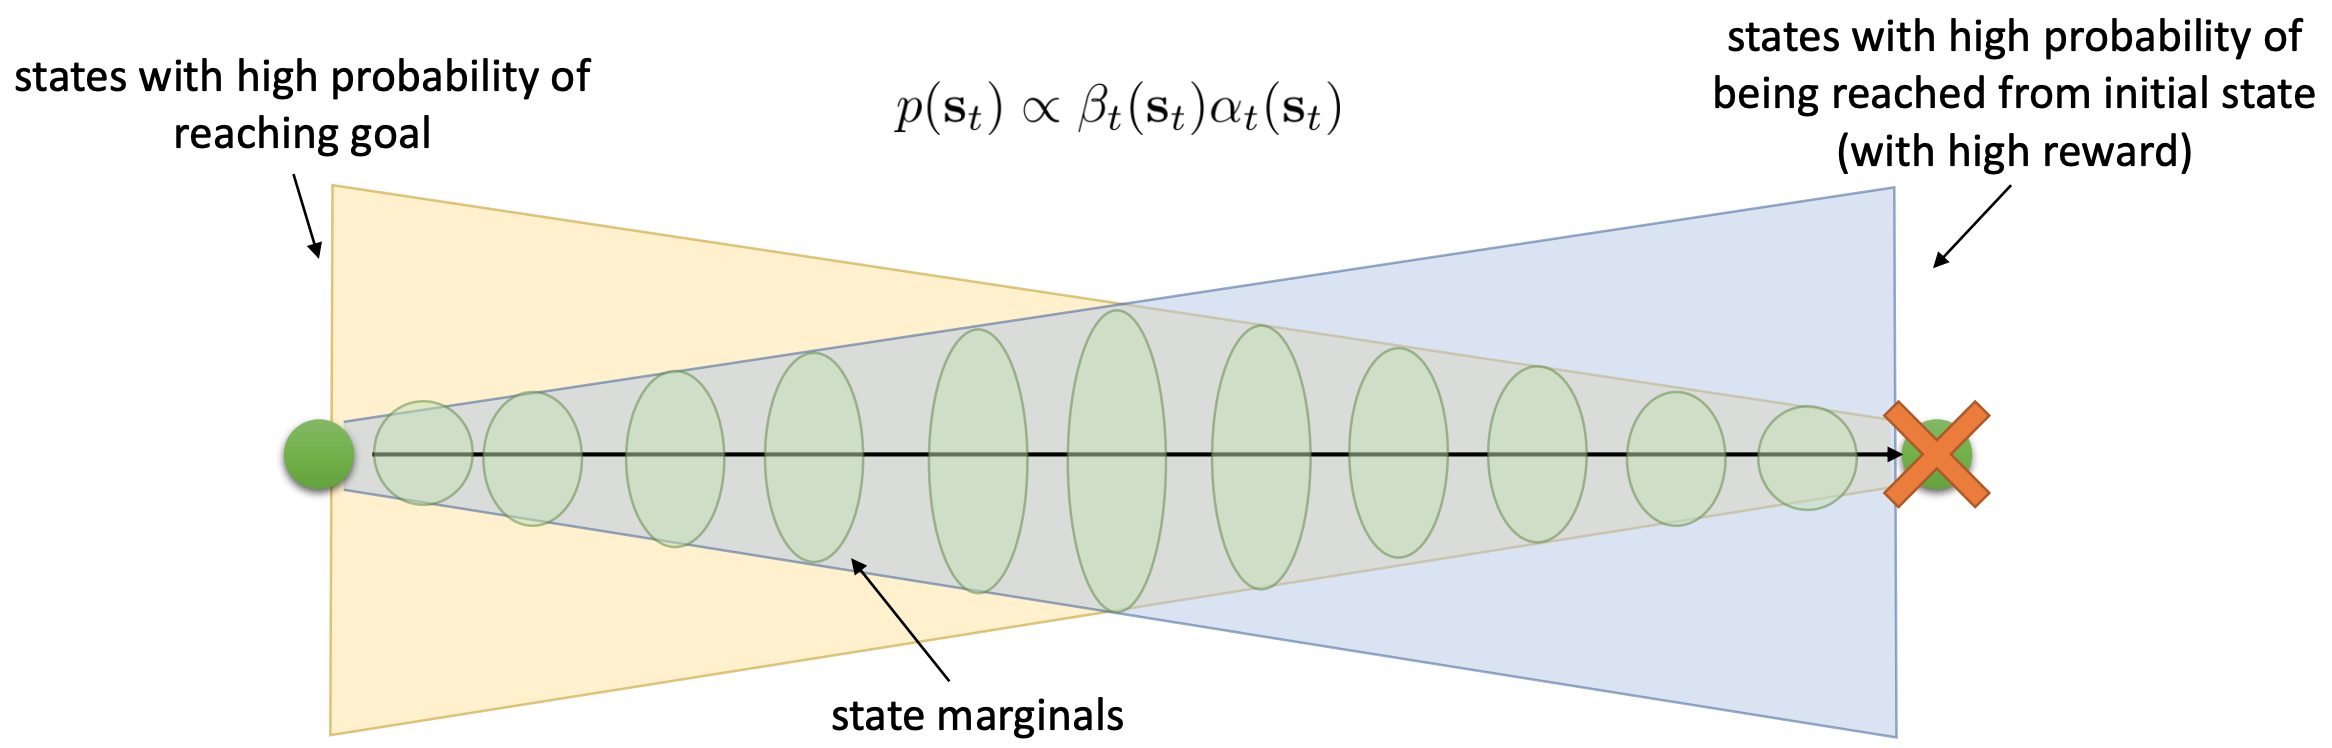
\includegraphics[scale=0.4]{figures/marginal.png}
    \caption{Forward/backward messages intersection}
    \label{fig:marginal}
\end{figure}

\section{The Optimism Problem}
Recall in the dynamic programming view of our backward message inference, the Q-function can be written as:
\[
Q_t(s_t,a_t) = r(s_t,a_t) + \log \mathbb{E}[\exp (V_{t+1}(s_{t+1}))]
\]
We have shown that $\log\mathbb{E}\exp$ behaves like a $\max$, thus bringing us bias in the estimate of Q-function. Marginalizing and conditioning the backward message $\beta_t(s_t,a_t) = p(\mathcal{O}_{t:T}|s_t,a_t)$, we can have two different distributions to infer: first, we can have the policy $p(a_t|s_t,\mathcal{O}_{1:T})$, which means given that you had a high reward (optimal), what was your action probability? Second, we can have the transition $p(s_{t+1}|s_t,a_t,\mathcal{O}_{1:T})$, and we should notice that this is not equal to the transition probability $p(s_{t+1}|s_t,a_t)$ because now we are asking given that you obtained high rewards, what was your transition probability? To address the optimism problem, we need to ask the first question: given that you obtained high reward, what was your action probability, assuming that we have the same transition probability, such that we are no luckier than we usually are. 

It turns out the first question is a difficult one. To answer that question, we can find another distribution $q(s_{1:T},a_{1:T})$ that is close to $p(s_t,a_t|\mathcal{O}_{1:T})$, but have the same $p(s_{t+1}|s_t,a_t)$. So let's us try variational inference. Let our evidence $x$, what we have observed, be the optimality variables $\mathcal{O}_{1:T}$, and the latent variable $z$, what we have not observed, be the trajectory $s_{1:T},a_{1:T}$. Using variational inference, we find a $q(z)$ to approximate $p(z|x)$.

Let $q(s_{1:T},a_{1:T}) = p(s_1)\prod_t p(s_{t+1}|s_t,a_t)q(a_t|s_t)$ since we are keeping the same initial state distribution and the same transition. Recall that the variational lower bound of the likelihood approximation is:
\[
\log p(x)\geq \mathbb{E}_{z\sim q(z)}[\log p(x,z) - \log q(z)]
\]
plugging in our previous definition of $q(z)$, we have
\begin{align*}
    \log p(\mathcal{O}_{1:T}) &\geq \mathbb{E}_{(s_{1:T},a_{1:T})\sim q}\bigg[ \log p(s_1) + \sum_{t=1}^T \log p(s_{t+1}|s_t,a_t) + \log p(\mathcal{O}_{T}|s_t,a_t)\\ &- \log p(s_1) - \sum_{t=1}^T \log p(s_{t+1}|s_t,a_t) - \sum_{t=1}^T\log q(a_t|s_t) \bigg]\\
    &= \mathbb{E}_{(s_{1:T},a_{1:T})\sim q}\left[\sum_t r(s_t,a_t) - \log q(a_t|s_t)\right]\\
    &= \mathbb{E}_{(s_{1:T},a_{1:T})\sim q}\left[r(s_t,a_t)+\mathcal{H}(q(a_t|s_t))\right]
\end{align*}
Therefore, to maximize the lower bound, we maximize the reward and the entropy.

%fill this in later
Using dynamic programming, we can get rid of the optimism $\max$ in the Bellman backup term.